\begin{pastexam}[label={px:ncku-115-ee-ds-01}]{成大電機所 115 學年度 第 1 題}
（問答）

\textbf{Problem 1: Priority Queue (20 pts)}

\textit{A hospital emergency department treats patients based on urgency (severity score).}
\begin{enumerate}[label=(\alph*)]
\item \textbf{[4 pts]} In terms of Time Complexity, state the primary advantage of using a Priority
Queue over a standard FIFO Queue for finding the next patient to treat.
\item \textbf{[4 pts]} Assume a \textbf{Max-Heap}. Insert the following patients in this order
(Severity Scores):
\[ P1(3),\quad P2(5),\quad P3(2),\quad P4(4) \]
\textbf{Draw the final heap structure} (tree view) below.
\item \textbf{[2 pts]} Starting from the result in (b), show the \textbf{array representation} of the
heap after two \texttt{extract-max} operations have been performed.
\item \textbf{[6 pts]} The time complexity of Heap operations is determined by the tree structure.
Answer the following:
\begin{enumerate}[label=\arabic*.]
\item What is the \textbf{height} of a binary heap with $n$ nodes?
\item In a worst-case \texttt{Insert}, how many swaps occur relative to the height?
\item If we used a \textbf{Sorted Array} instead, what would be the complexity of \texttt{Insert}?
\end{enumerate}
\item \textbf{[4 pts]} To prevent ``starvation'' of low-severity patients, the system increases a
patient's priority based on wait time. Name or briefly describe \textbf{one} mechanism to implement
this efficiently.
\end{enumerate}
\end{pastexam}

\begin{pastsoln}
$n$ 是等候中的病人數。

\textbf{(a)} 一般的 FIFO 佇列只依到達的先後排，要找出「最緊急」的病人，必須把佇列裡 $n$ 個人全部看一遍，
$O(n)$，取出後還要把中間的空位補起來。 優先佇列用二元堆積實作時，最緊急的病人永遠在根：查看是
$O(1)$，取出（extract-max）和加入新病人（insert）都是 $O(\log n)$（資結書第~8.1~、8.3~節）。 主要優點：
找下一位病人從 $O(n)$ 降到 $O(\log n)$。

\textbf{(b)} 最大堆積用陣列存，位置從 $1$ 編號，$i$ 的父節點是 $\lfloor i/2 \rfloor$。 插入放在最後一格，比
父節點大就往上交換（上浮，資結書虛擬碼~8.2）。
\begin{center}
\begin{tabular}{lll}
\toprule
插入 & 上浮的過程 & 陣列 \\
\midrule
P1(3) & 第一個元素，直接當根 & $[3]$ \\
P2(5) & 放在位置 2；$5 > 3$（位置 1），交換 & $[5, 3]$ \\
P3(2) & 放在位置 3；$2 < 5$，不動 & $[5, 3, 2]$ \\
P4(4) & 放在位置 4；$4 > 3$（位置 2），交換；$4 < 5$，停 & $[5, 4, 2, 3]$ \\
\bottomrule
\end{tabular}
\end{center}
\begin{center}
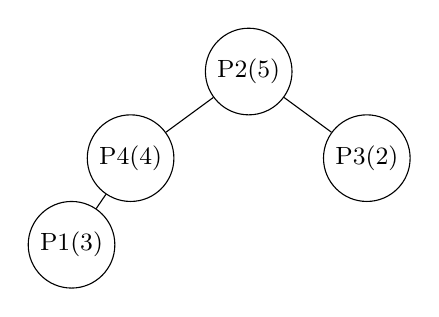
\begin{tikzpicture}[level distance=11mm,every node/.style={circle,draw,minimum size=11mm,inner sep=0pt,font=\small},
  level 1/.style={sibling distance=30mm},level 2/.style={sibling distance=15mm}]
\node {P2(5)} child {node {P4(4)} child {node {P1(3)}} child[missing]} child {node {P3(2)}};
\end{tikzpicture}
\end{center}

\textbf{(c)} extract-max：取出根，最後一格搬到根，再往下沉（和較大的子節點交換）。
\begin{itemize}
\item 第一次：取出 P2(5)，最後一格的 P1(3) 搬到根，得 $[3, 4, 2]$；$3$ 的子節點 $4$、$2$ 中 $4$ 較大且 $> 3$，
交換，得 $[4, 3, 2]$。
\item 第二次：取出 P4(4)，最後一格的 P3(2) 搬到根，得 $[2, 3]$；子節點 $3 > 2$，交換，得 $[3, 2]$。
\end{itemize}
陣列是 $[3, 2]$，也就是 $[\text{P1}(3), \text{P3}(2)]$。

\textbf{(d)}
\begin{enumerate}
\item $n$ 個節點的二元堆積是完整二元樹，高度（數邊）是 $\lfloor \log_2 n \rfloor$，也就是 $\Theta(\log n)$。
（照資結書數節點的定義是 $\lfloor \log_2 n \rfloor + 1$。）
\item 最壞情況新元素比所有祖先都大，從最底層一路上浮到根，每一層交換一次，交換次數等於高度
$\lfloor \log_2 n \rfloor$（新元素放進去之後的高度），所以 Insert 是 $O(\log n)$。
\item 排好序的陣列：用二分搜尋找插入位置只要 $O(\log n)$，但要把後面的元素都往後挪一格，最壞
挪 $n$ 個，Insert 是 $O(n)$。 （好處是取出最大值 $O(1)$：放在陣列尾端直接拿。）
\end{enumerate}

\textbf{(e)} 這叫\textbf{老化}（aging）：等越久，優先權越高。 一個有效率的做法是把優先權寫成
\[
p(t) = s + \alpha\,(t - a),
\]
$s$ 是嚴重程度，$a$ 是到達時間，$t$ 是現在的時間，$\alpha > 0$ 是每單位等候時間加多少分。 關鍵是
$\alpha t$ 對所有病人都一樣，比較兩位病人時會消掉：$p_1(t) > p_2(t)$ 若且唯若 $s_1 - \alpha a_1 > s_2 -
\alpha a_2$。 所以堆積裡直接用\textbf{不隨時間改變}的鍵 $k = s - \alpha a$ 排序就好，病人到達時算一次，
之後完全不用更新，insert、extract-max 仍是 $O(\log n)$。

如果加分的方式不是線性的（例如等超過 30 分鐘就升一級），可以改用可以改鍵的索引堆積（資結書
第~8.3~節虛擬碼~8.4）：定期把等候超過門檻的病人做 increase-key，每次 $O(\log n)$。 不要每隔一段時間把
所有病人的優先權都改一遍再重建堆積，那樣每次要 $O(n)$。
\end{pastsoln}
